\subsection{拓展实验 E：批次级权衡在全天是否成立}

\begin{figure*}[t]
	\centering
	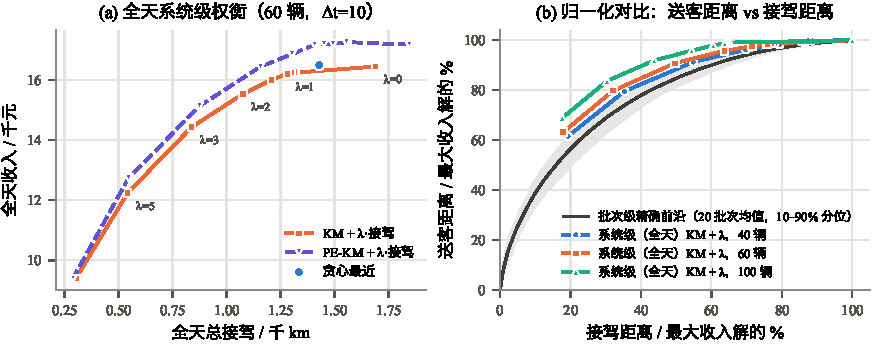
\includegraphics[width=\textwidth]{fig/exp7_system_front.pdf}
	\caption{(a) 在 KM / PE-KM 边权中加入接驾惩罚 $\lambda\cdot2p_{dj}$ 后的全天收入–总接驾距离（10 个测试日均值）；(b) 以最大收入解为 100\% 归一化后，批次级精确前沿与全天系统级曲线的对比}
	\label{fig:system}
\end{figure*}

实验二与拓展 A 都在单个批次内讨论“收入–接驾”的权衡。但平台真正关心的是全天累计的指标，单批次的前沿是否反映系统层面的代价，需要另行检验。为此在全天仿真中把边权改为 $w_{dj}=\text{fare}_j-\lambda\cdot2p_{dj}$（$\lambda=1$ 表示 1\,km 接驾与 1\,km 送客等价），扫描 $\lambda\in[0,8]$，分别作用于 KM 即时收入和表格 PE-KM（$\beta=0.6$），$\Dt\in\{5,10,20\}$，三种车队。

\textbf{全天层面的权衡远比单批次平缓。} \Cref{fig:system}(b) 中，三条全天曲线都位于批次级精确前沿的上方。在单个批次内，把接驾距离压缩 20\% 平均要损失 3.0\% 的送客距离，压缩 35\% 要损失 7.7\%。在全天层面，KM 只需取 $\lambda=0.25$，接驾总距离就下降 12\%/22\%/35\%（40/60/100 辆），而收入只变化 $-0.0$\%/$-1.2$\%/$-1.1$\%。换成 PE-KM，同一 $\lambda$ 下接驾下降 11\%–25\%，收入反而上升 0.1\%–0.5\%；40 辆车、$\lambda=0.5$ 时收入上升 1.0\%。$\Dt=5$ 与 20 分钟时结论相同：在全部 12 种（$\Dt$，车队，基础策略）组合下，$\lambda=0.25$ 使接驾下降 8\%–35\%，收入变化在 $-1.2$\% 至 $+0.5$\% 之间。直到 $\lambda\ge2$，即接驾惩罚开始切断大量正收益的边，收入才明显下降（$\lambda=2$ 时 $-4$\% 至 $-6$\%，$\lambda=3$ 时 $-10$\% 至 $-13$\%）。

\textbf{原因是批次之间的替代与运力回收。} 单批次前沿假设“这一批没派的订单就丢了”。但订单耐心（20 分钟）不短于批次间隔，被远处司机放弃的订单往往在本批次由近处司机接走，或在下一批次被其他司机服务，批次级的收入损失大部分在后续批次中被收回。另一方面，接驾时间本身占用运力：缩短接驾使司机更早空闲，在运力紧张时直接转化为更多的服务单量。这与网约车经济学中“空驶追单”（wild goose chase）的论断一致\cite{castillo2017surge}。最近贪心在 60/100 辆时接驾距离比 KM 短 15\%/34\%，收入差距却在 $\pm$1.7\% 以内，也印证了这一点。

由此得出一个实际的结论：以批次级帕累托前沿上的代价来权衡乘客体验和平台收入，会把真实代价\textbf{高估数倍}。在本仿真中，存在一段近乎“免费”的区间（$\lambda\approx0.25$–1），可以显著缩短接驾而几乎不损失收入。多目标派单应在系统层面评估，而不仅仅在单个批次上求前沿。
